\section{Virtual Labs}
Virtual Labs is an initiative by the Ministry of Human Resource Development (MHRD), Government of India, under the aegis of the National Mission on Education through Information and Communication Technology (NMEICT). This is coordinated by 12 participating institutes of which IIIT Hyderabad is a part. The main goal is to make any lab or education available independently of the platform. Virtual Labs mainly help professors and students who do not have proper lab facilities available by virtually emulating the scenario. \\
One of the current challenges faced by Virtual Labs is the ability to run code. This is mainly because of the requirement of a backend server to run the code. As the number of students using Virtual Labs increases, the load on the backend server increases. This is mainly because of the fact that the code will be run on the server and the results are sent back to the client. This would take a toll on the resources of the server. \\
The solution to this problem is to run the code on the client side. This would eliminate the need for a backend server, and possibly also allow interacting with the lab without any network after the first time. \\
For the scope of this paper, we would be working on a Python based Virtual Lab and we will be using pyodide as a base for our study and implementation. \\

\begin{figure}
    \centering
    \subcaptionbox{Server Side Compiling}
        {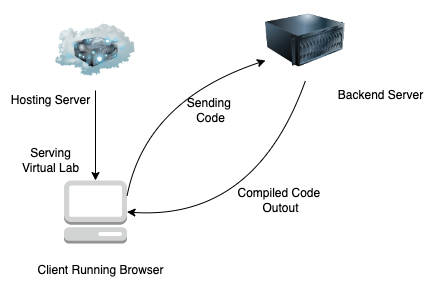
\includegraphics[width=0.55\textwidth]{images/server-model.png}}
    \subcaptionbox{Client Side Compiling}
        {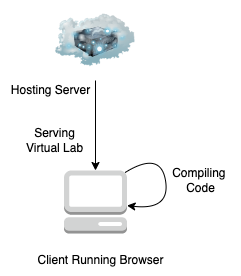
\includegraphics[width=0.35\textwidth]{images/client-model.png}}
    \caption{Server Side Model vs Client Side Model}
    \label{fig:csr vs ssr}
\end{figure}
